% ==========================================
% LatexRefinement Step Output: step4-05-12-25-tuesday-all-offset-final-copy8.tex
% Model: gemini-3.5-flash
% Temperature: 0.33
% TopP: 0.95
% TopK: 40
% MaxOutputTokens: 65535
% ThinkingBudget: 32765
% ThinkingLevel: HIGH
% Prompt Tokens: 48'140
% Candidates Tokens: 22'076 (inkl. Thinking Tokens)
% Cached Tokens: 0
% Processed on: 2026-07-18 12:30:37
% ==========================================

\lecturechapter[12]{Dienstag}{12. Mai}{12. Mai 2026}{Elementare Zahlentheorie: Euklidischer Algorithmus, Primzahlen und Modularrechnen}
% Old chapter title: Der euklidische Algorithmus

\begin{nice-box}[Vorlesungsübersicht \& Kontext]
In dieser Vorlesung steigen wir in die elementare Zahlentheorie über den ganzen Zahlen $\mathbb{Z}$ ein. Wir erarbeiten uns fundamentale Werkzeuge und Konzepte, die sowohl theoretisch als auch kryptografisch von zentraler Bedeutung sind:
\begin{itemize}
    \item \textbf{Teilbarkeit und Division mit Rest:} Die mathematische Grundlage für die Struktur der ganzen Zahlen.
    \item \textbf{Der euklidische Algorithmus:} Ein hocheffizientes Verfahren zur Bestimmung des größten gemeinsamen Teilers ($\operatorname{ggT}$) und dessen Darstellung als Linearkombination (Lemma von Bézout).
    \item \textbf{Primzahlen und der Hauptsatz der Arithmetik:} Die Existenz und Eindeutigkeit der Primfaktorzerlegung sowie die Unendlichkeit der Primzahlen.
    \item \textbf{Modularrechnen:} Die Einführung von Kongruenzrelationen, Restklassen und deren Verträglichkeit mit den Ringoperationen.
\end{itemize}
\end{nice-box}

\section{Der euklidische Algorithmus}
\subsection{Notation und Teilbarkeit}

\begin{spoken-clean}[00:00:00 - 00:01:49]
Hallo zusammen, wir fangen an. Wir gehen jetzt über zum nächsten Kapitel. Okay, ich folge jetzt der Kapitelstruktur im Skript, aber wir machen das hier ein bisschen anders oder kürzer als im Skript.

Also jetzt machen wir diese und nächste Woche, wahrscheinlich auch noch die übernächste, noch ein wenig elementare Zahlentheorie --- aber wirklich sehr elementar. Es ist also keine sehr tiefgehende Zahlentheorie, aber doch so viel, wie man auf jeden Fall im ersten Jahr gesehen haben sollte. Und einiges haben Sie wahrscheinlich auch bereits gesehen.

Im Skript gibt es da auch noch viel zu diesen Kettenbrüchen. Das ist zwar ein interessantes Thema --- insbesondere geht es um die Frage, wie man reelle Zahlen durch rationale Zahlen approximieren kann und was es da für Möglichkeiten gibt ---, aber wir machen jetzt wirklich nur etwas über die ganzen Zahlen. Wenn Sie das interessiert, sind Sie herzlich eingeladen, das noch durchzulesen. Aber ja, wir machen es jetzt ganz elementar.

In der Zahlentheorie interessiert man sich ja für die ganzen Zahlen oder sogar für die natürlichen Zahlen. Und okay, wir machen jetzt eine Notation in diesem Kapitel --- ich folge jetzt auch wieder dem Skript ---: Wir schreiben $\mathbb{N}$ für die natürlichen Zahlen, also $\{0, 1, 2, 3, \dots\}$.
\end{spoken-clean}

\begin{math-stroke}[Notation der natürlichen Zahlen]
\begin{notation}[Natürliche Zahlen]\label[notation]{not:natuerliche-zahlen}
Wir bezeichnen die Menge der \newterm{natürlichen Zahlen} mit:
\[ \mathbb{N} := \{0, 1, 2, 3, \dots\} \]
\end{notation}
\end{math-stroke}

\begin{spoken-clean}[00:01:49 - 00:03:53]
Der wichtige Punkt ist, dass hier die $0$ auch drin ist. Wir hatten vorher einmal angenommen, dass das gleich $\omega$ ist. Nun, $\omega$ verwendet man in der Regel nur in der Logik oder wenn man von Kardinalitäten und Ähnlichem spricht; in der restlichen Mathematik spricht man von den natürlichen Zahlen. Und okay, oft verwendet man dieses Symbol, oder früher hat man es oft verwendet.

Das Problem mit dem $\mathbb{N}$ für die natürlichen Zahlen is, dass nicht klar ist, was gemeint ist. Es ist vielleicht etwa --- ich weiß auch nicht --- die Hälfte der Leute, die sagt, dass die $0$ nicht dazugehört, und die andere Hälfte sagt, dass die $0$ dazugehört. Ich habe da keine starke Meinung, aber es gibt Leute mit sehr starken Meinungen dazu. Ich mache es aber so, wie es im Skript steht: dass die $0$ mit dabei ist. Das ist so, ja...

Ich bin mir bezüglich der Geschichte nicht ganz sicher. Ich glaube, irgendwann im letzten Jahrhundert hatten mal Mathematiker in Frankreich die Idee, dass das eine gute Idee ist, die $0$ dazuzunehmen. Und dadurch, dass das sehr gute Mathematiker waren, hat sich das durchaus gewissermaßen durchgesetzt; aber es gibt immer noch viele, die die $0$ nicht dazuzählen.

Das hat jetzt zur Folge, dass man das Symbol eigentlich gar nicht mehr richtig verwenden kann, weil eben nicht klar ist, was gemeint ist. Wenn ich also ein Paper schreibe --- und viele Leute machen das so ---, schreibt man oft einfach $\mathbb{Z}_{>0}$ oder $\mathbb{Z}_{\ge 0}$ oder Ähnliches. Dann ist direkt klar, was gemeint ist. Man muss nicht erst definieren, dass $\mathbb{N}$ dieses oder jenes ist, denn wenn man später irgendeinen Satz aus der Mitte des Papers anschaut, ist es sonst nicht mehr klar. Okay. Also genau: Das Symbol ist eigentlich fast zerstört in der heutigen Mathematik, eben weil es nicht mehr eindeutig definiert ist.
\end{spoken-clean}

\begin{math-stroke}[Eindeutige Bezeichnungen für Zahlenmengen]
Um Unklarheiten bezüglich der Zahl $0$ zu vermeiden, verwendet man in mathematischen Publikationen häufig folgende Bezeichnungen:
\begin{itemize}
    \item \textbf{Positive ganze Zahlen:} $\mathbb{Z}_{>0} := \{1, 2, 3, \dots\}$
    \item \textbf{Nichtnegative ganze Zahlen:} $\mathbb{Z}_{\ge 0} := \{0, 1, 2, 3, \dots\}$
\end{itemize}
\end{math-stroke}

\begin{spoken-clean}[00:03:53 - 00:05:44]
Gut. Okay, jetzt zu einer ganz einfachen Definition: Wir schauen uns jetzt ganze Zahlen an. Seien $a$ und $b$ ganze Zahlen. Wir sagen, dass $a$ die Zahl $b$ teilt --- oder auch, dass $b$ ein Vielfaches von $a$ ist ---, falls ein $c \in \mathbb{Z}$ existiert, sodass $b = a \cdot c$ ist. Und wir verwenden, weil wir das so oft schreiben, einfach die Notation $a \mid b$ --- also $a$ senkrechter Strich $b$ ---, das haben Sie bestimmt auch schon gesehen.
\end{spoken-clean}

\begin{math-stroke}[Definition der Teilbarkeit]
\begin{definition}[Teilbarkeit]\label[definition]{def:teilbarkeit}
Seien $a, b \in \mathbb{Z}$. Wir sagen \newterm{$a$ teilt $b$} (oder $b$ ist ein \newterm{Vielfaches} von $a$), falls ein $c \in \mathbb{Z}$ existiert, sodass:
\[ b = a \cdot c \]
Notation: $a \mid b$.
\end{definition}
\end{math-stroke}

\begin{spoken-clean}[00:05:44 - 00:07:09]
Und das ist das Schöne an den ganzen Zahlen! Das ist ja das, was die ganzen Zahlen so spannend macht: dass gewisse Zahlen einander teilen und andere nicht. Das hat man in einem Körper ja nicht --- in einem Körper teilt alles alles, solange es nicht null ist. Das ist das Schöne an einem Körper --- beziehungsweise, ein Körper ist aus anderen Gründen schön ---, aber ja, das macht die ganzen Zahlen sehr interessant. Und wie Sie wissen, führt das sehr, sehr schnell zu äußerst schwierigen Fragen, die sehr tief gehen und die man auch heute immer noch nicht ganz versteht.
\end{spoken-clean}

\begin{didactic-insight}[Die algebraische Struktur der Teilbarkeit]
Im Gegensatz zu einem Körper $K$ (wie $\mathbb{Q}$ oder $\mathbb{R}$), in dem jedes von Null verschiedene Element ein multiplikatives Inverses besitzt und somit die Teilbarkeitsrelation trivial ist (für alle $a, b \in K \setminus \{0\}$ gilt $a \mid b$), bildet der Ring der ganzen Zahlen $\mathbb{Z}$ eine reichhaltige Struktur. Die Existenz von Nicht-Einheiten führt direkt zur Definition von Primzahlen und wirft fundamentale Fragen der Zahlentheorie auf.
\end{didactic-insight}

\subsection{Teilen mit Rest}

\begin{spoken-clean}[00:07:09 - 00:12:02]
Gut, machen wir als Nächstes eine einfache Proposition oder ein Lemma: das Teilen mit Rest. Sehr nützlich! Wenn wir eine natürliche Zahl $a$ (wobei $a \neq 0$) haben und $b$ eine beliebige ganze Zahl ist, dann existieren eindeutige ganze Zahlen $q$ und $r$, sodass gilt: $b = a \cdot q + r$, wobei dieses $r$ größer gleich $0$, aber strikt kleiner als $a$ ist.

Okay, das ist das, was Sie schon in der Grundschule machen: Teilen mit Rest. Man schaut also, wie oft $a$ in $b$ hineinpasst, und dann bleibt eben noch ein Rest übrig, der aber strikt kleiner als $a$ ist. Aber ja, das ist relativ zentral, und dass man das in den ganzen Zahlen so machen kann, ist eine sehr schöne Eigenschaft.
\end{spoken-clean}

\begin{math-stroke}[Teilen mit Rest]
\begin{proposition}[Teilen mit Rest]\label[proposition]{prop:teilen-mit-rest}
Sei $a \in \mathbb{N} \setminus \{0\}$ und $b \in \mathbb{Z}$. Dann existieren eindeutige $q, r \in \mathbb{Z}$, sodass:
\[ b = a \cdot q + r \quad \text{mit} \quad 0 \le r < a \]
\end{proposition}
\end{math-stroke}

\begin{student-interaction}[Studentenfrage]
Wenn $a$ gleich $0$ ist?
\end{student-interaction}

\begin{spoken-clean}[00:12:02 - 00:13:37]
Ja, also ich habe bestimmt auch angenommen, dass $a$ nicht $0$ ist. Das ist ja die Aussage, die wir beweisen wollen. Genau, also nehmen wir an, dass $a$ nicht $0$ sein darf. Wenn $a$ gleich $0$ wäre, dann würden wir etwas Widersprüchliches beweisen --- das geht natürlich nicht. $a$ kann nicht $0$ sein. Ja, gute Bemerkung! Genau. Ja, ich... ja, genau, das wird...

Genau, eben, das würde sonst nicht existieren, weil wir ja schon angenommen haben, dass $a$ ungleich $0$ ist. Wenn $a$ doch $0$ wäre, dann würden wir etwas Widersprüchliches beweisen. Das geht nicht, $a$ kann nicht $0$ sein. Ja, gute Bemerkung. Ja, gute Bemerkung. Ja, ich... ja, genau.

Machen wir einfach $a \neq 0$, ich glaube, das ist gut. Wenn $a = 0$ ist, ja... dann kann man... ja, machen wir $a \neq 0$, sonst geht es nicht. Das macht sonst wenig Sinn. Danke!
\end{spoken-clean}

\begin{meta-note}[Korrektur auf der Tafel]
Der Dozent korrigiert die Formulierung der Proposition auf der Tafel und schränkt die natürliche Zahl $a$ auf $a \in \mathbb{N} \setminus \{0\}$ ein.
\end{meta-note}

\subsection{Der größte gemeinsame Teiler}

\begin{spoken-clean}[00:13:37 - 00:17:09]
Okay, dann machen wir das Nächste: den größten gemeinsamen Teiler. Nächste Proposition --- das haben Sie vielleicht auch schon gesehen ---: Wir nehmen $a$ und $b$ als natürliche Zahlen, aber diesmal nicht beide gleich $0$. Machen wir das so. Dann existiert --- um ganz sicher zu sein --- eine eindeutige natürliche Zahl $d \in \mathbb{N}$, sodass gilt: Erstens, $d \mid a$ und $d \mid b$. Und das Zweite ist: Für alle natürlichen Zahlen $k$, sodass $k \mid a$ und $k \mid b$ gilt, folgt $k \mid d$. Also jeder andere gemeinsame Teiler teilt auch $d$.

Okay, und dann schreiben wir noch außerdem --- okay, so eine Zahl existiert ---, dass $x$ und $y$ in $\mathbb{Z}$ existieren, sodass $d = a \cdot x + b \cdot y$ ist. Okay, also $d$ lässt sich als ganzzahlige Linearkombination von $a$ und $b$ darstellen.
\end{spoken-clean}

\begin{math-stroke}[Der größte gemeinsame Teiler]
\begin{proposition}[Größter gemeinsamer Teiler und Lemma von Bézout]\label[proposition]{prop:ggt-bezout}
Seien $a, b \in \mathbb{N}$ mit $(a, b) \neq (0,0)$. Dann existiert ein eindeutiges $d \in \mathbb{N}$, sodass:
\begin{enumerate}[label=\textbf{(\roman*)}]
    \item $d \mid a$ und $d \mid b$ (\newterm{gemeinsamer Teiler}),
    \item für alle $k \in \mathbb{N}$ mit $k \mid a$ und $k \mid b$ gilt $k \mid d$.
\end{enumerate}
Zudem existieren $x, y \in \mathbb{Z}$, sodass:
\[ d = a \cdot x + b \cdot y \]
\end{proposition}

\begin{definition}[Größter gemeinsamer Teiler]\label[definition]{def:ggt}
Dieses eindeutig bestimmte $d$ heißt der \newterm{größte gemeinsame Teiler} von $a$ und $b$.
\[ \text{Notation: } d = \operatorname{ggT}(a, b) \quad (\text{engl. } \operatorname{gcd}(a, b)) \]
\end{definition}
\end{math-stroke}

\subsection{Beweise der Sätze}

\begin{proof}[Beweis von \cref{prop:ggt-bezout}]
\begin{spoken-clean}[00:17:09 - 00:18:28]
Okay, und der Beweis ist sehr direkt. Wir schreiben das jetzt ein bisschen hochgestochener auf, als man eigentlich müsste: Wir definieren eine Menge $S$ als alle Zahlen der Form $a \cdot u + b \cdot v$, wobei $u, v \in \mathbb{Z}$ sind, und wir nehmen nur diejenigen davon, die größer als $0$ sind. Aus dieser Menge nehmen wir einfach das minimale Element $d$. Das geht, weil wir in den natürlichen Zahlen sind und diese ja wohlgeordnet sind.

Und okay, wenn wir so ein $d \in S$ haben, sagen wir noch, nehmen wir noch ein $x$ und $y$ in $\mathbb{Z}$, sodass wir schreiben können: $d = a \cdot x + b \cdot y$. Genau, und dieses $d$ ist ja größer als $0$, weil es zu den positiven natürlichen Zahlen gehört. Okay, jetzt zeigen wir zuerst, dass $d$ ein Teiler von $a$ und $b$ ist.
\end{spoken-clean}

\begin{math-stroke}[Beweis der Existenz des ggT]
\begin{ai-proof-skeleton-invisible-content}
% 1. Definiere S als Menge aller positiven Linearkombinationen au + bv.
% 2. Zeige S ist nicht leer und wähle minimales d in S.
% 3. Zeige d teilt a und d teilt b mittels Division mit Rest.
% 4. Zeige jeder gemeinsame Teiler k teilt d.
% 5. Zeige Eindeutigkeit von d.
\end{ai-proof-skeleton-invisible-content}

Wir definieren die Menge aller positiven ganzzahligen Linearkombinationen von $a$ und $b$:
\[ S := \{ a \cdot u + b \cdot v \mid u, v \in \mathbb{Z} \} \cap \mathbb{N}_{>0} \]
Da $(a, b) \neq (0,0)$, ist $S \neq \emptyset$ (beispielsweise ist $a^2 + b^2 \in S$). Da $S \subseteq \mathbb{N}$ und die natürlichen Zahlen wohlgeordnet sind, besitzt $S$ ein minimales Element $d \in S$.
Da $d \in S$, existieren $x, y \in \mathbb{Z}$, sodass:
\[ d = a \cdot x + b \cdot y \]
\end{math-stroke}

\begin{spoken-clean}[00:18:28 - 00:22:20]
Dieses minimale Element --- das ist sehr direkt. Wir teilen $a$ mit Rest durch $d$. Also wir schreiben: $a = d \cdot q + r$ mit $0 \le r < d$. Und dann können wir schreiben: Was ist $r$? $r = a - d \cdot q$. Jetzt setzen wir die Definition von $d$ ein, das ist $a - (a \cdot x + b \cdot y) \cdot q$. Und das kann man jetzt umschreiben, das gibt $a(1 - x \cdot q) + b(-y \cdot q)$.

Und das ist wieder von dieser Form, oder? Das ist eine ganzzahlige Linearkombination von $a$ und $b$. Das heißt, dieses $r$ gehört auch wieder in diese Menge $S$, oder es ist gleich $0$. Aber wir haben ja angenommen, dass $d$ minimal in $S$ ist. Und da $r$ strikt kleiner als $d$ ist, kann $r$ nicht in $S$ liegen. Das heißt, die einzige Möglichkeit ist, dass $r = 0$ ist. Und das bedeutet $a = d \cdot q$, sprich $d \mid a$. Und analog zeigt man, dass $d$ auch $b$ teilt.
\end{spoken-clean}

\begin{math-stroke}[Nachweis der Teilbarkeit]
Wir teilen $a$ mit Rest durch $d$:
\[ a = d \cdot q + r \quad \text{mit} \quad 0 \le r < d \]
Wir drücken den Rest $r$ aus:
\begin{align*}
r &= a - d \cdot q \\
&= a - (a \cdot x + b \cdot y) \cdot q \\
&= a(1 - x \cdot q) + b(-y \cdot q)
\end{align*}
Dies zeigt, dass $r$ ebenfalls eine ganzzahlige Linearkombination von $a$ und $b$ ist.
\begin{itemize}
    \item Wäre $r > 0$, so würde $r \in S$ gelten. Da jedoch $r < d$, stünde dies im Widerspruch zur Minimalität von $d \in S$.
    \item Folglich muss $r = 0$ sein, woraus $a = d \cdot q$ und somit $d \mid a$ folgt.
\end{itemize}
Völlig analog zeigt man durch Division von $b$ durch $d$, dass auch $d \mid b$ gilt. Somit ist $d$ ein gemeinsamer Teiler von $a$ und $b$.
\end{math-stroke}

\begin{spoken-clean}[00:22:20 - 00:23:34]
Okay, und aus dieser Behauptung können wir jetzt die Proposition ableiten.
\end{spoken-clean}

\begin{math-stroke}[Nachweis der Teilbarkeit durch andere Teiler]
Sei $k \in \mathbb{N}$ ein beliebiger gemeinsamer Teiler von $a$ und $b$, d.\,h. $k \mid a$ und $k \mid b$.
Dann existieren $m, n \in \mathbb{Z}$ mit $a = k \cdot m$ und $b = k \cdot n$. Wir setzen dies in die Darstellung von $d$ ein:
\begin{align*}
d &= a \cdot x + b \cdot y \\
&= (k \cdot m) \cdot x + (k \cdot n) \cdot y \\
&= k \cdot (m \cdot x + n \cdot y)
\end{align*}
Da $m \cdot x + n \cdot y \in \mathbb{Z}$, folgt unmittelbar $k \mid d$.
\end{math-stroke}

\begin{spoken-clean}[00:23:34 - 00:25:45]
Okay, und dazu nehmen wir an, dass es zwei solche $d$ gibt. Nehmen wir an, wir haben ein $d$ und ein $d'$ in $\mathbb{N}$, sodass beide diese Bedingungen erfüllen. Daraus folgt natürlich, wenn die zwei diese Bedingungen erfüllen, dass $d \mid d'$ und $d' \mid d$ gilt. Aber $d$ und $d'$ sind ja in den natürlichen Zahlen. Und falls $d \mid d'$ und $d' \mid d$ gilt, dann folgt daraus direkt, dass $d = d'$ ist. Das heißt, der größte gemeinsame Teiler ist eindeutig, und somit haben wir die Eindeutigkeit gezeigt.

Relativ direkt, das heißt, das ist alles klar. Also die Aussage ist ja eigentlich auch schon klar, wenn man das so aufschreibt. Das weiß man auch schon aus der Grundschule, dass der größte gemeinsame Teiler eindeutig ist. Das ist also keine große Überraschung. Ja.
\end{spoken-clean}

\begin{math-stroke}[Eindeutigkeit des ggT]
Seien $d, d' \in \mathbb{N}$ zwei Zahlen, die die Bedingungen \textbf{(i)} und \textbf{(ii)} erfüllen.
\begin{itemize}
    \item Da $d$ ein gemeinsamer Teiler ist und $d'$ Bedingung \textbf{(ii)} erfüllt, gilt $d \mid d'$.
    \item Da $d'$ ein gemeinsamer Teiler ist und $d$ Bedingung \textbf{(ii)} erfüllt, gilt $d' \mid d$.
\end{itemize}
Da $d, d' \in \mathbb{N}$, folgt aus $d \mid d'$ und $d' \mid d$ sofort $d = d'$.
\end{math-stroke}
\end{proof}

\begin{student-interaction}[Studentenfrage zur Definition]
Ist es aber nicht ganz unten in der Proposition, wenn $a=0$ ist...
\end{student-interaction}

\begin{spoken-clean}[00:25:45 - 00:26:09]
Ah! Ja, genau! Wenn $a=0$ ist, dann... ja, ich habe bestimmt auch angenommen, dass $a$ nicht $0$ ist. Das ist ja die Aussage, die wir beweisen wollen. Genau, also nehmen wir an, dass $a$ nicht $0$ sein darf. Wenn $a$ gleich $0$ wäre, dann würden wir etwas Widersprüchliches beweisen --- das geht natürlich nicht. $a$ kann nicht $0$ sein. Ja, gute Bemerkung! Genau. Ja, ich... ja, genau, das wird...

Genau, eben, das würde sonst nicht existieren, weil wir ja schon angenommen haben, dass $a$ ungleich $0$ ist. Wenn $a$ doch $0$ wäre, dann würden wir etwas Widersprüchliches beweisen. Das geht nicht, $a$ kann nicht $0$ sein. Ja, gute Bemerkung. Ja, gute Bemerkung. Ja, ich... ja, genau.

Machen wir einfach $a \neq 0$, ich glaube, das ist gut. Wenn $a = 0$ ist, ja... dann kann man... ja, machen wir $a \neq 0$, sonst geht es nicht. Das macht sonst wenig Sinn. Danke!
\end{spoken-clean}

\begin{student-interaction}[Studentenfrage]
...wenn ich diese Menge definiert habe, einmal $b$, einmal $a$ da drin...
\end{student-interaction}

\begin{spoken-clean}[00:26:09 - 00:26:19]
Ja, $a$ und $b$ sind beide in diesem $I$ enthalten, das ist so, ja.
\end{spoken-clean}

\begin{student-interaction}[Studentenfrage]
Und wenn nachher $d$ die minimale... Grad 1... Grad $a$ oder $b$ ist...
\end{student-interaction}

\begin{spoken-clean}[00:26:21 - 00:26:25]
Grad $a$ oder $b$ ist. Genau, absolut.
\end{spoken-clean}

\begin{student-interaction}[Studentenfrage]
Aber $a$ und $b$... aber $a$ nicht ein Vielfaches von $b$ ist...
\end{student-interaction}

\begin{spoken-clean}[00:26:26 - 00:26:36]
Nein, das kann man nicht finden, nein. Weil sonst könnten Sie es voneinander subtrahieren, und dann...
\end{spoken-clean}

\begin{student-interaction}[Studentenfrage]
...wenn $a$ gleich $2$ ist und $b$ gleich $3$...
\end{student-interaction}

\begin{spoken-clean}[00:26:37 - 00:26:40]
Ja, genau, dann ist das $d$ gleich $1$.
\end{spoken-clean}

\begin{student-interaction}[Studentenfrage]
$2$ nachher auch...
\end{student-interaction}

\begin{spoken-clean}[00:26:41 - 00:27:34]
Ist auch drin, aber ist nicht minimal, genau. Da haben Sie $3 - 2$, das ist dann drin, und das ist $1$.

Also $I$ sind alle ganzzahligen... $I$ haben wir gesagt... in Ihrem Beispiel haben wir $I$ als die Menge aller $2u + 3v$, wobei $u, v \in \mathbb{Z}$ sind, geschnitten mit den positiven natürlichen Zahlen. Und das wäre jetzt zum Beispiel genau $\{1, 2, 3, \dots\}$. Okay?

Wenn Sie $u = -1$ nehmen und $v = 1$, dann haben Sie da $2 \cdot (-1) + 3 \cdot 1 = 1$. Also der Fall, dass dieses $d$ genau das Kleinere von den beiden ist (vorausgesetzt, beide sind ungleich $0$), das entspricht genau dem Fall, wo eine Zahl die andere teilt. Äh, ja.
\end{spoken-clean}

\begin{student-interaction}[Studentenfrage]
Gibt es kleinere...
\end{student-interaction}

\begin{spoken-clean}[00:27:35 - 00:28:27]
Äh, ja, muss man ein bisschen überlegen. Da könnte man zum Beispiel... könnte man zum Beispiel $2 \cdot 5 - 3 \cdot 3$... Okay, ja. Es funktioniert tatsächlich immer.

Okay. Also ich bin nicht ganz überzeugt von den Argumenten, aber sonst... Es muss so sein, das ist genau der kleinste gemeinsame Teiler. Weil eben gerade... genau, weil es minimal ist. Genau mit dem Argument kann man zeigen: Wenn Sie einen gemeinsamen Teiler finden, dann muss es dieser sein.
\end{spoken-clean}

\begin{math-stroke}[Beispiel zur minimalen Linearkombination]
Für $a = 2$ und $b = 3$ betrachten wir die Menge $I$:
\[ I = \{ 2u + 3v \mid u, v \in \mathbb{Z} \} \cap \mathbb{N}_{>0} = \{1, 2, 3, \dots\} \]
Das minimale Element dieser Menge ist $d = 1$, da für $u = -1$ und $v = 1$ gilt:
\[ 2 \cdot (-1) + 3 \cdot 1 = 1 \]
\end{math-stroke}

\section{Der euklidische Algorithmus}

\subsection{Funktionsweise des euklidischen Algorithmus}

\begin{spoken-clean}[00:28:27 - 00:30:44]
Wir werden gleich noch sehen, wie man diesen $\operatorname{ggT}$ dann auch berechnet: Das ist der euklidische Algorithmus.

Das ist wirklich einer der sehr schönen... Sie kennen von Euklid die \qt{Elemente}, ein fantastisches Werk, das über $2000$ Jahre alt und eigentlich weiterhin aktuell ist. Klar, man hat heute ein bisschen andere Begriffe von Axiomatik und so weiter, aber im Wesentlichen ist das... also es war eigentlich bahnbrechend als Buch. Dass es immer noch aktuell ist, zeigt die Beständigkeit der Mathematik, und es ist wirklich brillant, was er darin macht. Wenn Sie mal Zeit haben, ein bisschen in den \qt{Elementen} von Euklid zu lesen --- das ist sehr, sehr nett und weiterhin verständlich. Man muss sich natürlich ein bisschen in die Sprache einlesen, aber es ist wirklich ein sehr schönes Buch --- beziehungsweise viele Bücher natürlich.

Es ist auch extrem einflussreich; ich glaube, man kann fast nicht unterschätzen, wie einflussreich das auf die gesamte Mathematik und die Naturwissenschaften als Ganzes war.

Okay, wie dem auch sei: Darin beschreibt er einen Algorithmus, um diesen $\operatorname{ggT}$ zu finden. Er macht das natürlich in einem geometrischen Kontext --- er nimmt zwei verschiedene Längen und beschreibt einen Algorithmus, wie man eine Länge findet, die beide Längen misst ---, aber es ist genau das, was wir hier machen. Und so wie ich es verstehe, ist das weiterhin der Algorithmus der Wahl, der verwendet wird, um den $\operatorname{ggT}$ von zwei Zahlen zu finden. In Computerprogrammen in der Informatik kommt es durchaus vor, dass man den $\operatorname{ggT}$ benötigt, und das wird mit dem euklidischen Algorithmus gemacht.
\end{spoken-clean}

\begin{spoken-clean}[00:30:44 - 00:33:37]
Was wir da haben, sind zwei ganze Zahlen $a$ und $b$, und wir nehmen an, $a$ ist kleiner als $b$. Wenn sie gleich sind, dann haben wir den $\operatorname{ggT}$ ja schon direkt.

Und okay, was wir eigentlich machen: Wir teilen sukzessive mit Rest. Wir können schreiben: Seien $q_1, \dots, q_{n+1} \in \mathbb{Z}$ und $0 \le r_n < r_{n-1} < \dots < r_1 < a$, sodass... Also ich schreibe das jetzt ein bisschen... so wie ich es aufgeschrieben habe, ist es ein bisschen wie Reverse Engineering, weil man das eigentlich umgekehrt macht.

Man macht das umgekehrt: Was man macht, ist Teilen mit Rest. Wir schreiben $b$ auf und teilen es durch $a$ mit Rest, dann haben wir $b = a \cdot q_1 + r_1$. Und was wir als Nächstes machen: Wir teilen $a$ durch diesen Rest $r_1$, ebenfalls wieder mit Rest. Also schreiben wir $a$ als $r_1 \cdot q_2$, was uns einen weiteren Rest $r_2$ gibt. Und dann teilen wir wieder $r_1$ durch diesen Rest $r_2$. Wir schreiben $r_1 = r_2 \cdot q_3$ plus ein weiterer Rest $r_3$. Und das machen wir immer so weiter, bis wir zu $r_{n-2} = r_{n-1} \cdot q_n + r_n$ kommen.

Und diese Reste werden natürlich immer kleiner: $r_1$ ist strikt kleiner als $a$, $r_2$ ist strikt kleiner als $r_1$, $r_3$ ist strikt kleiner als $r_2$. Das heißt, die Reste werden immer strikt kleiner, bleiben aber immer größer gleich $0$. Daher muss dieser Prozess irgendwann aufhören, das kann nicht endlos weitergehen. Irgendwann haben wir dann den Fall, dass $r_{n-1}$ einfach ein Vielfaches von $r_n$ ist.

Okay, und der euklidische Algorithmus besteht einfach darin, dass man dieses Teilen mit Rest immer weiter durchführt, bis es nicht mehr weitergeht, und...
\end{spoken-clean}

\begin{math-stroke}[Der euklidische Algorithmus]
Seien $a, b \in \mathbb{N}$ mit $a < b$ \inlinemetanote{[Anmerkung: Hier muss $a > 0$ vorausgesetzt werden, da sonst der erste Divisionsschritt $b = a \cdot q_1 + r_1$ nicht durchführbar ist (Division durch Null)]}. Wir führen sukzessive Divisionen mit Rest durch. Es existieren $q_1, \dots, q_{n+1} \in \mathbb{Z}$ und Reste $r_1, \dots, r_n \in \mathbb{N}$ mit:
\[ 0 \le r_n < r_{n-1} < \dots < r_1 < a \]
sodass:
\begin{align}
b &= a \cdot q_1 + r_1 \label{eq:euclid-step1} \\
a &= r_1 \cdot q_2 + r_2 \label{eq:euclid-step2} \\
r_1 &= r_2 \cdot q_3 + r_3 \label{eq:euclid-step3} \\
&\,\,\vdots \nonumber \\
r_{n-2} &= r_{n-1} \cdot q_n + r_n \label{eq:euclid-step-n-1} \\
r_{n-1} &= r_n \cdot q_{n+1} \label{eq:euclid-step-n}
\end{align}
\end{math-stroke}

\begin{spoken-clean}[00:33:37 - 00:34:13]
Die Behauptung ist, dass der $\operatorname{ggT}$ von $a$ und $b$ genau $r_n$ ist. Also dieses $r_n$, das man am Ende erhält, wo der Rest dann $0$ ergibt, das ist der größte gemeinsame Teiler von $a$ und $b$.
\end{spoken-clean}

\begin{math-stroke}[Behauptung zum euklidischen Algorithmus]
\begin{theorem}[Korrektheit des euklidischen Algorithmus]\label[theorem]{thm:euclid-correctness}
Der letzte von Null verschiedene Rest $r_n$ im euklidischen Algorithmus ist der größte gemeinsame Teiler von $a$ und $b$:
\[ \operatorname{ggT}(a, b) = r_n \]
\end{theorem}
\end{math-stroke}

\begin{proof}[Beweis von \cref{thm:euclid-correctness}]

\subsection{Korrektheitsbeweis des euklidischen Algorithmus}

\begin{spoken-clean}[00:34:13 - 00:37:41]
Und ja, das ist das, was Euklid bereits beobachtet hat. Machen wir den Beweis. Man könnte es auch als ein allgemeines Prinzip beschreiben: Der Witz hier ist eigentlich, dass der $\operatorname{ggT}(a, b)$ dasselbe ist wie der $\operatorname{ggT}(a, r_1)$. Also quasi, wenn man von $b$ ein Vielfaches von $a$ abzieht, dann ändert das den größten gemeinsamen Teiler von $a$ und $b$ nicht.

Und das geht dann immer so weiter. Dann haben wir wieder: Der $\operatorname{ggT}(a, r_1)$ ist wiederum das Gleiche wie der $\operatorname{ggT}(r_1, r_2)$, und am Schluss hat man dann das Ergebnis. Es ist einfach diese Beobachtung. Schreiben wir das ein bisschen auf.

Wir haben, dass der $\operatorname{ggT}(a, b) \mid a$ und der $\operatorname{ggT}(a, b) \mid b$ gilt. Per Definition teilt er $b$, aber er teilt auch $a$ und somit auch alle Vielfachen von $a$ und folglich auch deren Differenz. Okay, das heißt, er teilt auch $r_1$. Er teilt sowohl $a$ als auch $r_1$. Und somit folgt, dass der $\operatorname{ggT}(a, b)$ ein Teiler von $\operatorname{ggT}(a, r_1)$ ist.

Okay. Aber wir haben auch das Umgekehrte: Wir haben, dass der $\operatorname{ggT}(a, r_1) \mid a$ gilt, und der teilt natürlich auch alle Vielfachen von $a$, also auch $a \cdot q_1$. Und er teilt auch $a \cdot q_1 + r_1$, aber das ist genau dasselbe wie $b$. Das heißt, dieser $\operatorname{ggT}$ teilt sowohl $a$ als auch $b$, was bedeutet, dass er auch den $\operatorname{ggT}(a, b)$ teilt. Okay? Das heißt, wir haben: Der $\operatorname{ggT}(a, r_1)$ teilt auch den $\operatorname{ggT}(a, b)$."

Und somit folgt: Wenn der eine den anderen teilt und umgekehrt, dann müssen sie gleich sein. Das heißt, genau dieser $\operatorname{ggT}$ zwischen $a$ und $b$ ist derselbe wie der $\operatorname{ggT}$ zwischen $a$ und $r_1$. Dasselbe Argument kann man jetzt Schritt für Schritt machen, und dann erhalten wir genau das, was wir suchen.
\end{spoken-clean}

\begin{math-stroke}[Beweis der Korrektheit des euklidischen Algorithmus]
Wir zeigen zunächst, dass der größte gemeinsame Teiler invariant unter Division mit Rest ist, d.\,h. $\operatorname{ggT}(a, b) = \operatorname{ggT}(a, r_1)$.
\begin{itemize}
    \item \textbf{Richtung 1 ($\operatorname{ggT}(a, b) \mid \operatorname{ggT}(a, r_1)$):}
    Nach Definition gilt $\operatorname{ggT}(a, b) \mid a$ und $\operatorname{ggT}(a, b) \mid b$. Da $r_1 = b - a \cdot q_1$ eine ganzzahlige Linearkombination ist, folgt:
    \[ \operatorname{ggT}(a, b) \mid (b - a \cdot q_1) \implies \operatorname{ggT}(a, b) \mid r_1 \]
    Da $\operatorname{ggT}(a, b)$ sowohl $a$ als auch $r_1$ teilt, teilt er auch deren größten gemeinsamen Teiler:
    \[ \operatorname{ggT}(a, b) \mid \operatorname{ggT}(a, r_1) \]
    
    \item \textbf{Richtung 2 ($\operatorname{ggT}(a, r_1) \mid \operatorname{ggT}(a, b)$):}
    Umgekehrt gilt $\operatorname{ggT}(a, r_1) \mid a$ und $\operatorname{ggT}(a, r_1) \mid r_1$. Da $b = a \cdot q_1 + r_1$, folgt:
    \[ \operatorname{ggT}(a, r_1) \mid (a \cdot q_1 + r_1) \implies \operatorname{ggT}(a, r_1) \mid b \]
    Da $\operatorname{ggT}(a, r_1)$ sowohl $a$ als auch $b$ teilt, teilt er auch deren größten gemeinsamen Teiler:
    \[ \operatorname{ggT}(a, r_1) \mid \operatorname{ggT}(a, b) \]
\end{itemize}
Da beide Teiler in $\mathbb{N}$ liegen, folgt aus der gegenseitigen Teilbarkeit die Gleichheit:
\[ \operatorname{ggT}(a, b) = \operatorname{ggT}(a, r_1) \]

Wendet man dieses Argument sukzessive auf alle Schritte \eqref{eq:euclid-step1}--\eqref{eq:euclid-step-n} des Algorithmus an, erhält man die Gleichheitskette:
\[ \operatorname{ggT}(a, b) = \operatorname{ggT}(a, r_1) = \operatorname{ggT}(r_1, r_2) = \dots = \operatorname{ggT}(r_{n-1}, r_n) \]
Da im letzten Schritt $r_{n-1} = r_n \cdot q_{n+1}$ gilt, ist $r_n$ ein Teiler von $r_{n-1}$. Somit ist:
\[ \operatorname{ggT}(r_{n-1}, r_n) = r_n \]
Dies beweist die Behauptung $\operatorname{ggT}(a, b) = r_n$.
\end{math-stroke}

\begin{spoken-clean}[00:37:41 - 00:38:39]
Ganz ähnlich beweist man, dass $\operatorname{ggT}(a, r_1)$ dasselbe ist wie $\operatorname{ggT}(r_1, r_2)$ und so weiter. Und okay, $r_{n-1}$ ist einfach ein Vielfaches von $r_n$, das heißt, der $\operatorname{ggT}$ ist genau $r_n$. Okay, und das ist genau das, was wir behauptet hatten.
\end{spoken-clean}

\begin{math-stroke}[Analytische Gleichheitskette]
Völlig analog lässt sich die Gleichheit für jeden weiteren Schritt zeigen:
\[ \operatorname{ggT}(a, r_1) = \operatorname{ggT}(r_1, r_2) = \dots = \operatorname{ggT}(r_{n-1}, r_n) = r_n \]
\end{math-stroke}
\end{proof}

\begin{spoken-clean}[00:38:39 - 00:40:35]
Gut, wir können noch ein Beispiel machen. Ich glaube, das kann man fast selbst mit dem Taschenrechner ausrechnen, aber...

Sagen wir zum Beispiel: Was ist der $\operatorname{ggT}$ von $2026$ und --- was hatte ich aufgeschrieben? --- $226$?

Dann sehen wir: Okay, fangen wir an. $2026 = 226 \cdot 8 + 218$. Okay, und dann sieht man: $226 = 218 \cdot 1 + 8$. Und dann sieht man, dass $218 = 8 \cdot 27 + 2$ ist. Und schließlich sehen wir: $8 = 2 \cdot 4 + 0$. Okay?"

Das heißt, wir erhalten, dass der größte gemeinsame Teiler von $2026$ und $226$ gleich $2$ ist.

Okay, das hätte man jetzt vermutlich auch direkt sehen können, weil $2026 = 2 \cdot 1013$ ist und $1013$ eine Primzahl ist, wie man zeigen kann. Zudem sind beide Zahlen gerade. Aber der euklidische Algorithmus funktioniert wirklich immer, und es geht meistens auch relativ schnell. Die Zahlen werden sehr schnell kleiner, also können Sie die $\operatorname{ggT}$s gut von Hand ausrechnen.
\end{spoken-clean}

\begin{math-stroke}[Beispiel zum euklidischen Algorithmus]
\begin{example}[Berechnung von $\operatorname{ggT}(2026, 226)$]\label[example]{ex:euclid-example}
Wir bestimmen den größten gemeinsamen Teiler von $2026$ und $226$ mittels des euklidischen Algorithmus:
\begin{align*}
2026 &= 226 \cdot 8 + 218 \\
226 &= 218 \cdot 1 + 8 \\
218 &= 8 \cdot 27 + 2 \\
8 &= 2 \cdot 4 + 0
\end{align*}
Der letzte von Null verschiedene Rest ist $2$. Folglich gilt:
\[ \operatorname{ggT}(2026, 226) = 2 \]
\end{example}
\end{math-stroke}

\begin{spoken-clean}[00:40:35 - 00:40:39]
Okay, machen wir eine Pause und danach weiter mit Primzahlen.
\end{spoken-clean}

\begin{lecture-break}[15-minütige Vorlesungspause]
Die Vorlesung wird nach einer kurzen Pause fortgesetzt. Der Dozent bereitet die Tafel für das nächste Thema (Primzahlen) vor.
\end{lecture-break}

\section{Primzahlen}
\subsection{Definition und Grundeigenschaften}

\begin{spoken-clean}[00:40:39 - 00:42:16]
Das ist die folgende Definition, die Sie auch schon kennen: Wir sagen, dass eine Zahl $p \in \mathbb{N}$ eine Primzahl ist, falls $p$ genau zwei positive Teiler hat, nämlich $p$ und $1$.

Okay, und das ist wichtig: genau zwei! Die $1$ ist also keine Primzahl, weil die $1$ nur einen einzigen positiven Teiler hat, nämlich sich selbst. Also eine Primzahl --- oder wir sagen oft auch einfach: $p$ ist prim.

Okay, und das ist die geläufige Definition für die natürlichen Zahlen.
\end{spoken-clean}

\begin{math-stroke}[Definition der Primzahl]
\begin{definition}[Primzahl]\label[definition]{def:primzahl}
Eine Zahl $p \in \mathbb{N}$ heißt \newterm{Primzahl} (oder kurz: \newterm{prim}), falls $p$ genau zwei positive Teiler besitzt, nämlich $1$ und $p$.
\end{definition}

\begin{remark}[Die Zahl 1]\label[remark]{rem:zahl-eins}
Die Zahl $1$ ist definitionsgemäß \emph{keine} Primzahl, da sie nur einen einzigen positiven Teiler besitzt (nämlich sich selbst).
\end{remark}
\end{math-stroke}

\begin{spoken-clean}[00:42:16 - 00:43:14]
Es gibt allerdings eigentlich eine bessere Charakterisierung --- das ist die folgende Eigenschaft ---, aber für die natürlichen Zahlen läuft das auf dasselbe hinaus. Das ist die folgende Proposition:

Sei $p \in \mathbb{N}$ eine Primzahl und seien $a, b$ ganze Zahlen. Falls $p$ das Produkt $a \cdot b$ teilt, dann teilt $p$ entweder $a$ oder $p$ teilt $b$.
\end{spoken-clean}

\begin{math-stroke}[Das Lemma von Euklid]
\begin{proposition}[Lemma von Euklid]\label[proposition]{prop:lemma-von-euklid}
Sei $p \in \mathbb{N}$ eine Primzahl und seien $a, b \in \mathbb{Z}$. Falls $p \mid a \cdot b$, so gilt:
\[ p \mid a \quad \text{oder} \quad p \mid b \]
\end{proposition}
\end{math-stroke}

\begin{proof}[Beweis von \cref{prop:lemma-von-euklid}]

\subsection{Beweis des Lemmas von Euklid}

\begin{spoken-clean}[00:43:14 - 00:46:03]
Okay, und wenn Sie Algebra machen --- als nächsten Schritt, was auch für beliebige Ringe gilt ---, da schaut man sich auch solche Faktorisierungsfragen an, und dann definiert man Primelemente eher über diese Eigenschaft. Aber für uns ist das das Gleiche.

Okay, beweisen wir diese Proposition. Wir nehmen an, dass $p \mid a \cdot b$ gilt. Wenn $p \mid a$ gilt, dann sind wir fertig. Wir nehmen jetzt also an, dass $p$ die Zahl $a$ nicht teilt. Was bedeutet das, dass $p$ die Zahl $a$ nicht teilt? Okay.

Wenn $p$ kein Teiler von $a$ ist, was muss dann der $\operatorname{ggT}$ von $p$ und $a$ sein? Ja, genau $1$. Weil $p$ ja nur zwei Teiler hat: $p$ und $1$. Das heißt, der $\operatorname{ggT}$ zwischen $p$ und $a$ muss entweder $p$ oder $1$ sein. Aber wenn er $p$ wäre, würde das bedeuten, dass $p$ die Zahl $a$ teilt. Da das nicht the Fall ist, muss es $1$ sein. Okay.

Daraus folgt mit dem, was wir vorher gesehen haben: Es existieren ganze Zahlen $x, y \in \mathbb{Z}$ mit $a \cdot x + p \cdot y = 1$. Okay.

Und jetzt können wir einfach auf beiden Seiten mit $b$ multiplizieren. Auf der rechten Seite erhalten wir $b$. Das heißt, $b = (a \cdot b) \cdot x + p \cdot b \cdot y$. Das ist einfach diese Gleichung, multipliziert auf beiden Seiten mit $b$.

Und jetzt sehen wir: Dieser Term hier ist durch $p$ teilbar, weil er ein Vielfaches von $p$ ist. Dieser andere Teil ist aber auch durch $p$ teilbar, weil hier das Produkt $a \cdot b$ steht, das ja nach Voraussetzung von $p$ geteilt wird. Das heißt, auch die Summe und somit $b$ ist durch $p$ teilbar. Und das ist genau das, was wir zeigen wollten.
\end{spoken-clean}

\begin{math-stroke}[Beweis des Lemmas von Euklid]
\begin{ai-proof-skeleton-invisible-content}
% 1. Nimm an, p teilt ab und p teilt nicht a.
% 2. Da p prim ist, sind die einzigen Teiler von p genau 1 und p. Da p nicht a teilt, muss ggT(p, a) = 1 sein.
% 3. Nach dem Lemma von Bézout existieren x, y in Z mit ax + py = 1.
% 4. Multipliziere mit b: b = abx + pby.
% 5. Da p | ab, teilt p den ersten Summanden abx. Da p | p, teilt p den zweiten Summanden pby.
% 6. Folglich teilt p die Summe, also p | b.
\end{ai-proof-skeleton-invisible-content}

Wir nehmen an, dass $p \mid a \cdot b$. Falls $p \mid a$ gilt, ist die Aussage bereits erfüllt. Wir nehmen daher an, dass $p \nmid a$.
Da $p$ eine Primzahl ist, sind ihre einzigen positiven Teiler $1$ und $p$. Da $p$ kein Teiler von $a$ ist, folgt für den größten gemeinsamen Teiler:
\[ \operatorname{ggT}(p, a) = 1 \]
Nach dem Lemma von Bézout (\cref{prop:ggt-bezout}) existieren ganze Zahlen $x, y \in \mathbb{Z}$, sodass:
\begin{equation}\label{eq:bezout-identity2}
a \cdot x + p \cdot y = 1
\end{equation}
Wir multiplizieren Gleichung \eqref{eq:bezout-identity2} auf beiden Seiten mit $b$:
\begin{equation}\label{eq:bezout-multiplied2}
b = (a \cdot b) \cdot x + p \cdot b \cdot y
\end{equation}
Wir untersuchen die Teilbarkeit der Summanden auf der rechten Seite von Gleichung \eqref{eq:bezout-multiplied2}:
\begin{itemize}
    \item Nach Voraussetzung gilt $p \mid a \cdot b$, woraus unmittelbar $p \mid (a \cdot b) \cdot x$ folgt.
    \item Offensichtlich gilt auch $p \mid p \cdot b \cdot y$.
\end{itemize}
Da $p$ beide Summanden teilt, teilt $p$ auch deren Summe, woraus folgt:
\[ p \mid b \]
Dies schließt den Beweis ab.
\end{math-stroke}
\end{proof}

\subsection{Der Hauptsatz der Arithmetik}

\begin{spoken-clean}[00:46:03 - 00:47:29]
Okay, dann schauen wir uns den Beweis des nächsten Satzes an. Das ist der, den Sie auch schon kennen: der Hauptsatz der Arithmetik --- oder auch Fundamentalsatz der Arithmetik.

Er besagt: Sei $a \in \mathbb{Z} \setminus \{0\}$. Dann gibt es ein $k \ge 0$ und Primzahlen $p_1, \dots, p_k$, sodass wir schreiben können: $a = c \cdot p_1 \cdots p_k$ mit $c \in \{1, -1\}$.

Wir können also jede ganze Zahl, die ungleich $0$ ist, als Produkt von Primzahlen schreiben.
\end{spoken-clean}

\begin{math-stroke}[Der Hauptsatz der Arithmetik]
\begin{theorem}[Hauptsatz der Arithmetik]\label[theorem]{thm:hauptsatz-der-arithmetik}
Sei $a \in \mathbb{Z} \setminus \{0\}$. Dann existiert eine bis auf die Reihenfolge der Faktoren eindeutige Darstellung der Form:
\[ a = c \cdot p_1 \cdot p_2 \cdots p_k \]
wobei $c \in \{1, -1\}$, $k \in \mathbb{N}$ (für $k=0$ ist dies das leere Produkt, welches als $1$ definiert ist) und $p_1, \dots, p_k$ Primzahlen sind mit:
\[ p_1 \le p_2 \le \dots \le p_k \]
\end{theorem}
\end{math-stroke}

\begin{proof}[Beweis des Hauptsatzes der Arithmetik]
\subsubsection{Existenz der Primfaktorzerlegung}

\begin{spoken-clean}[00:47:29 - 00:48:34]
Und außerdem ist diese Faktorisierung eindeutig --- natürlich bis auf eine Permutation der Faktoren. Wenn wir die Faktoren permutieren, ändert das ja nichts an der Eindeutigkeit. Also eindeutig bis auf die Reihenfolge der Primfaktoren.
\end{spoken-clean}

\begin{spoken-clean}[00:48:34 - 00:51:54]
Beweis. Okay, und der Beweis ist eigentlich ein Induktionsbeweis. Wir können annehmen, dass $a$ positiv ist, weil wir dieses Vorzeichen $c$ haben. Wenn wir es für alle positiven $a$ beweisen, dann stimmt es auch für alle negativen, indem wir einfach $c = -1$ wählen. Ohne Einschränkung der Allgemeinheit nehmen wir also an, dass $a$ positiv ist.

Gut. Wir zeigen zuerst die Existenz. Und wir machen jetzt einfach Induktion über $a$. Für $a = 1$ erhalten wir das leere Produkt, das entspricht $k = 0$, was als $1$ definiert ist. Jetzt nehmen wir an, wir haben es für alle kleineren natürlichen Zahlen schon gezeigt, und wir wollen es für das nächste $a$ beweisen.

Falls $a$ prim ist, dann sind wir fertig. Falls $a$ nicht prim ist, so existieren $b, b'$ in den natürlichen Zahlen, sodass $a = b \cdot b'$ mit $1 < b, b' < a$. Nach Induktionsvoraussetzung existieren Primfaktorzerlegungen für $b$ und $b'$. Wenn wir das Produkt dieser beiden Zerlegungen nehmen, erhalten wir direkt eine Primfaktorzerlegung für $a$.
\end{spoken-clean}

\begin{math-stroke}[Existenzbeweis der Primfaktorzerlegung]
Wir beweisen die Existenz der Primfaktorzerlegung mittels starker Induktion über $a \in \mathbb{N}_{>0}$:
\begin{itemize}
    \item \textbf{Induktionsanfang ($a = 1$):}
    Für $a = 1$ ist die Aussage erfüllt, da das leere Produkt ($k = 0$) als $1$ definiert ist.
    
    \item \textbf{Induktionsschritt ($a > 1$):}
    Wir nehmen an, dass jede natürliche Zahl $m$ mit $1 \le m < a$ eine Primfaktorzerlegung besitzt. Wir zeigen die Behauptung für $a$:
    \begin{itemize}
        \item \textbf{Fall 1 ($a$ ist prim):}
        Ist $a$ eine Primzahl, so ist die Behauptung mit $k = 1$ und $p_1 = a$ trivialerweise erfüllt.
        
        \item \textbf{Fall 2 ($a$ ist zusammengesetzt):}
        Ist $a$ keine Primzahl, so existieren echte Teiler $b, b' \in \mathbb{N}$ mit:
        \[ a = b \cdot b' \quad \text{wobei} \quad 1 < b, b' < a \]
        Da sowohl $b$ als auch $b'$ strikt kleiner als $a$ sind, können wir die Induktionsvoraussetzung auf beide Faktoren anwenden. Es existieren somit Primfaktorzerlegungen:
        \[ b = q_1 \cdots q_r \quad \text{und} \quad b' = q'_1 \cdots q'_s \]
        mit Primzahlen $q_i, q'_j$. Durch Multiplikation dieser Darstellungen erhalten wir eine Primfaktorzerlegung für $a$:
        \[ a = b \cdot b' = q_1 \cdots q_r \cdot q'_1 \cdots q'_s \]
        Durch Sortieren der Faktoren erhalten wir die gewünschte geordnete Darstellung.
    \end{itemize}
\end{itemize}
\end{math-stroke}

\subsubsection{Eindeutigkeit der Primfaktorzerlegung}

\begin{spoken-clean}[00:52:18 - 00:53:43]
Okay, das heißt, wir können jede Zahl als Produkt von Primzahlen schreiben. Jetzt wollen wir noch zeigen, dass diese Zerlegung eindeutig ist.

Nehmen wir an, dass wir eine Zahl als zwei verschiedene Produkte schreiben können. Wir müssen zeigen, dass diese beiden Zerlegungen übereinstimmen. Wir nehmen also an, dass $a = p_1 \cdots p_k$ ist, und das soll dasselbe sein wie $q_1 \cdots q_m$. Das sind zwei solche Primfaktorzerlegungen.
\end{spoken-clean}

\begin{math-stroke}[Ansatz zur Eindeutigkeit]
Wir nehmen an, wir haben zwei Primfaktorzerlegungen für eine Zahl $a \in \mathbb{N}_{>1}$:
\begin{equation}\label{eq:eindeutigkeit-ansatz-p3}
a = p_1 \cdot p_2 \cdots p_k = q_1 \cdot q_2 \cdots q_m
\end{equation}
wobei $p_1 \le p_2 \le \dots \le p_k$ und $q_1 \le q_2 \le \dots \le q_m$ Primzahlen sind.
\end{math-stroke}

\begin{spoken-clean}[00:53:43 - 00:56:08]
Und jetzt müssen wir zeigen, dass das dieselben Faktoren sind. Gut, aber dafür verwenden wir jetzt genau die vorherige Proposition. Sie sehen das, oder? Wir beginnen mit dem ersten Faktor $p_1$. Da $p_1$ das gesamte Produkt auf der rechten Seite teilt, muss es einen dieser Faktoren teilen. Und da diese Faktoren wiederum Primzahlen sind, müssen die beiden Primzahlen identisch sein.

Das heißt: Per Definition ist $p_1$ ein Teiler von $q_1 \cdot q_2 \cdots q_m$. Da $p_1$ prim ist, gilt gemäß der Proposition, dass $p_1$ ein Teiler von $q_i$ für ein gewisses $i$ sein muss. Und da $q_i$ prim ist, folgt daraus sofort $p_1 = q_i$. Aufgrund der Sortierung $q_1 \le q_2 \le \dots \le q_m$ gilt insbesondere $q_1 \le q_i = p_1$.
\end{spoken-clean}

\begin{math-stroke}[Teilbarkeit des ersten Faktors]
Da $p_1$ das Produkt $q_1 \cdots q_m$ teilt, folgt nach dem Lemma von Euklid (\cref{prop:lemma-von-euklid}), dass ein $i \in \{1, \dots, m\}$ existiert, sodass:
\[ p_1 \mid q_i \]
Da $q_i$ eine Primzahl ist, folgt zwingend $p_1 = q_i$. Aufgrund der Sortierung der Faktoren gilt:
\begin{equation}\label{eq:p1-q1-abschatzung}
q_1 \le q_i = p_1
\end{equation}
\end{math-stroke}

\begin{spoken-clean}[00:56:08 - 00:58:16]
Symmetrisch folgt durch Vertauschen der Rollen von $p$ und $q$, dass $q_1$ das Produkt $p_1 \cdots p_k$ teilt, woraus $q_1 = p_j$ für ein $j$ und somit $p_1 \le p_j = q_1$ folgt. Daraus ergibt sich unmittelbar $p_1 = q_1$.

Wir können diesen gemeinsamen Faktor auf beiden Seiten der Gleichung kürzen, das heißt: $p_2 \cdots p_k = q_2 \cdots q_m$. Nach Induktionsvoraussetzung ist diese verbleibende Zerlegung eindeutig, woraus $k - 1 = m - 1 \implies k = m$ sowie $p_i = q_i$ für alle $i$ folgt. Dies schließt den Beweis des Hauptsatzes der Arithmetik ab.

Gut. Ein sehr schöner Beweis! Den können Sie am Wochenende bei Kaffee und Kuchen auch Ihren Großeltern erklären.
\end{spoken-clean}

\begin{math-stroke}[Induktionsschritt und Abschluss]
Symmetrisch teilt $q_1$ das Produkt $p_1 \cdots p_k$, woraus $q_1 = p_j$ für ein $j \in \{1, \dots, k\}$ folgt. Es gilt:
\begin{equation}\label{eq:q1-p1-abschatzung}
p_1 \le p_j = q_1
\end{equation}
Aus \eqref{eq:p1-q1-abschatzung} und \eqref{eq:q1-p1-abschatzung} folgt:
\[ p_1 = q_1 \]
Wir kürzen diesen Faktor in \eqref{eq:eindeutigkeit-ansatz-p3}:
\[ p_2 \cdots p_k = q_2 \cdots q_m \]
\begin{explanation-of-steps}[Implizite Induktion]
Streng genommen führen wir hier eine vollständige Induktion über die Anzahl der Primfaktoren $k$ (oder alternativ über die Größe der Zahl $a$). Für $k=0$ (die Zahl $1$) ist die Eindeutigkeit trivial. Nehmen wir an, die Eindeutigkeit gilt für Produkte aus $k-1$ Primfaktoren. Durch das Kürzen von $p_1 = q_1$ betrachten wir nun die echt kleinere Zahl $a' = a / p_1 = p_2 \cdots p_k$. Diese hat nur noch $k-1$ Faktoren auf der linken Seite. Nach Induktionsannahme ist ihre Zerlegung eindeutig.
\end{explanation-of-steps}
Nach Induktionsannahme ist diese verbleibende Zerlegung eindeutig, woraus $k = m$ und $p_i = q_i$ für alle $i \in \{2, \dots, k\}$ folgt.
\end{math-stroke}
\end{proof}

\subsection{Beispiele und Komplexität der Primfaktorzerlegung}

\begin{spoken-clean}[00:58:16 - 01:00:35]
Hier noch Beispiele aus aktuellem Anlass: $2026 = 2 \cdot 1013$. Hier müssen wir einfach glauben, dass $1013$ eine Primzahl ist. Ich habe einen Freund, der Zahlentheoretiker ist und an Neujahr immer einen Glückwunschgruß für das neue Jahr verschickt, in dem er etwas zur Faktorisierung des aktuellen Jahres schreibt --- so bleibt man auf dem Laufenden. Es gibt aber auch relativ effiziente Tests, die entscheiden, ob eine Zahl eine Primzahl ist. Das ist gut. Bis zu ein paar Millionen kann man das auch einfach durchprobieren, das ist kein großes Problem.

Aber man kann auch bei sehr, sehr großen Zahlen mit sehr effizienten Algorithmen zumindest mit sehr hoher Wahrscheinlichkeit sagen, ob es Primzahlen sind. Vielleicht ist das nicht zu $100\,\%$ sicher, aber, wie soll man sagen, zu $99{,}99999\,\%$ sicher, dass es eine Primzahl ist --- und das geht in Sekundenschnelle. Das machen Computer tagtäglich tausendfach, wenn Sie auf HTTPS-Webseiten zugreifen.

Okay, und das Jahr $2025$ ist dann ein bisschen anders. Das kann man schreiben als... das ist ja durch $25$ teilbar: $3^4 \cdot 5^2$. Das heißt, ja, das ist einfach kurz für $3 \cdot 3 \cdot 3 \cdot 3 \cdot 5 \cdot 5$.
\end{spoken-clean}

\begin{math-stroke}[Beispiele zur Primfaktorzerlegung]
\begin{examples}[Faktorisierung aktueller Jahreszahlen]\label[examples]{ex:jahreszahlen}
Wir betrachten die Primfaktorzerlegungen der Jahre $2026$ und $2025$:
\begin{align*}
    2026 &= 2 \cdot 1013 \quad (\text{wobei } 1013 \text{ prim ist}) \\
    2025 &= 3^4 \cdot 5^2 = 3 \cdot 3 \cdot 3 \cdot 3 \cdot 5 \cdot 5
\end{align*}
\end{examples}
\end{math-stroke}

\begin{spoken-clean}[01:00:35 - 01:03:42]
Okay, um zu entscheiden, ob eine Zahl prim ist oder nicht, gibt es hocheffiziente Algorithmen --- zumindest probabilistische. Eine wichtige Bemerkung ist jedoch, dass es im Allgemeinen keine effizienten Algorithmen gibt, um diese Zerlegung tatsächlich zu finden.

Es ist sehr einfach, zwei Primzahlen miteinander zu multiplizieren --- das kann man sehr effizient machen, sogar von Hand, wenn die Zahlen nicht allzu lang sind. Aber das Umgekehrte, eine gegebene Zahl in ihre Primfaktoren zu zerlegen, ist extrem schwierig. Diesen Fakt kann man nutzen, um nützliche kryptografische Verschlüsselungsverfahren zu entwickeln. Und wenn irgendwann mal jemand einen solchen effizienten Algorithmus finden sollte, dann bemerken Sie das sehr bald, weil dann am nächsten Morgen Ihr Konto abgeräumt ist. Das ist effektiv so. Wir haben hoffentlich nächste Woche noch Zeit, um ein paar kryptografische Verfahren zu besprechen, die genau darauf beruhen.
\end{spoken-clean}

\begin{math-stroke}[Komplexitätsasymmetrie der Multiplikation und Faktorisierung]
\begin{remark}[Kryptografische Relevanz]\label[remark]{rem:kryptografie}
Während die Multiplikation zweier großer Primzahlen $p$ und $q$ rechnerisch extrem effizient ist, existiert für das umgekehrte Problem — die Bestimmung der Primfaktoren einer gegebenen zusammengesetzten Zahl $n = p \cdot q$ — nach heutigem Kenntnisstand kein effizienter (polynomialer) klassischer Algorithmus. Diese Asymmetrie bildet das Fundament moderner asymmetrischer Verschlüsselungsverfahren (wie RSA).
\end{remark}
\end{math-stroke}

\subsection{Die Unendlichkeit der Primzahlen}

\begin{spoken-clean}[01:03:42 - 01:05:53]
Okay, dann noch ein weiterer wichtiger und berühmten Satz, auch wieder von Euklid, den Sie bestimmt alle kennen: Es gibt unendlich viele Primzahlen.

Der Beweis ist ein sehr eleganter Widerspruchsbeweis. Wir nehmen an, es gäbe nur endlich viele Primzahlen. Dann können wir diese durchnummerieren: $p_1 < p_2 < \dots < p_r$. Und der schöne Trick ist nun: Wir betrachten die Zahl $n$, nämlich das Produkt all dieser endlich vielen Primzahlen $p_1 \cdots p_r$, und addieren $1$ dazu.

Jetzt wenden wir einfach den Hauptsatz der Arithmetik an und wissen, dass wir $n$ in Primfaktoren zerlegen können. Aber da sehen Sie, dass es ein Problem gibt, weil keine dieser Primzahlen $p_i$ dieses $n$ teilen kann.
\end{spoken-clean}

\begin{math-stroke}[Satz von Euklid]
\begin{theorem}[Satz von Euklid]\label[theorem]{thm:euklid-unendlich}
Es gibt unendlich viele Primzahlen.
\end{theorem}
\end{math-stroke}

\begin{proof}[Beweis des Satzes von Euklid]
\begin{spoken-clean}[01:05:53 - 01:07:28]
Daraus folgt mit dem Hauptsatz der Arithmetik, dass ein $j$ existiert, sodass diese Primzahl $p_j$ dieses $n$ teilt. Aber dann teilt $p_j$ auch $n$ minus das Produkt $p_1 \cdots p_r$ (das ja durch $p_j$ teilbar ist). Das ergibt aber einfach $1$. Und dann hätten wir eine Primzahl, die $1$ teilt, was ein offensichtlicher Widerspruch ist.

Das heißt, es muss unendlich viele Primzahlen geben. Ja, ein sehr schöner Beweis, den können Sie am Wochenende bei Kaffee und Kuchen auch Ihren Großeltern erklären.
\end{spoken-clean}

\begin{math-stroke}[Widerspruchsbeweis nach Euklid]
Angenommen, es gäbe nur endlich viele Primzahlen. Wir können diese der Größe nach ordnen:
\[ p_1 < p_2 < \dots < p_r \]
Wir betrachten die Zahl:
\begin{equation}\label{eq:euklid-zahl}
n = (p_1 \cdot p_2 \cdots p_r) + 1
\end{equation}
Nach dem Hauptsatz der Arithmetik (\cref{thm:hauptsatz-der-arithmetik}) besitzt $n$ mindestens einen Primfaktor $p_j \in \{p_1, \dots, p_r\}$, sodass $p_j \mid n$.
Da $p_j$ auch das Produkt $p_1 \cdots p_r$ teilt, teilt $p_j$ auch die Differenz:
\[ p_j \mid \bigl( n - (p_1 \cdot p_2 \cdots p_r) \bigr) \implies p_j \mid 1 \]
Dies steht im Widerspruch dazu, dass $p_j$ eine Primzahl (und somit $p_j > 1$) ist. Folglich existieren unendlich viele Primzahlen.
\end{math-stroke}
\end{proof}

\subsection{Verteilung von Primzahlen und der Primzahlsatz}

\begin{spoken-clean}[01:07:28 - 01:10:33]
Genau. Vielleicht noch eine Bemerkung, so als Fun Fact: In der Zahlentheorie ist es, wie Sie wissen, so, dass die Primzahlen immer noch ein Stück weit unverstanden sind. Es ist eine schöne, angenehme Mischung aus Mustern und ein bisschen Zufälligkeit. Und das ist natürlich etwas, was viele in der Mathematik fasziniert. Das andere ist, dass man sehr einfache, leicht zu verstehende, aber extrem schwierige Fragen stellen kann. Es gibt viele Fragen, die man sofort versteht, die aber immer noch offen sind. Das macht eine gewisse Faszination aus. Und es zeigt auch, dass die natürlichen Zahlen eine so grundlegende Struktur in der Mathematik sind, dass sie entsprechend kompliziert zu verstehen sind.

Vielleicht noch eine Bemerkung dazu, wie diese Primzahlen verteilt sind. Wir wissen ja: $2, 3, 5, 7$, dann gibt es $11, 13$, die nächste ist $17$. Es gibt schon immer weniger Primzahlen, je weiter man nach oben geht, das ist völlig richtig. Dazu gibt es eine wichtige Aussage: den Primzahlsatz. Wenn man die Funktion $\pi \colon \mathbb{R} \to \mathbb{N}$ betrachtet, die definiert ist als die Anzahl der Primzahlen kleiner gleich $x$ --- das können wir für jede reelle Zahl definieren ---, dann sieht das grafisch wie eine Treppenfunktion aus. Hier haben wir $\pi(x)$, hier haben wir $x$. Bis zur $2$ ist die Funktion $0$, bei $2$ springt sie auf $1$, bei $3$ geht sie nochmals eins hoch, bei $5$ wieder eins hoch, bei $7$ nochmals, bei $11$ und $13$ ebenso, und so weiter. Wenn man sich das im Großen anschaut, sieht man, dass die Kurve allmählich abflacht.
\end{spoken-clean}

\begin{math-stroke}[Die Primzahlzählfunktion \texorpdfstring{$\pi(x)$}{pi(x)}]
\begin{definition}[Primzahlzählfunktion]\label[definition]{def:primzahlzahlfunktion}
Die \newterm{Primzahlzählfunktion} $\pi \colon \mathbb{R} \to \mathbb{N}$ is definiert durch:
\[ \pi(x) = \bigl| \{ p \in \mathbb{N} \mid p \le x \land p \text{ ist prim} \} \bigr| \]
\end{definition}

\begin{center}
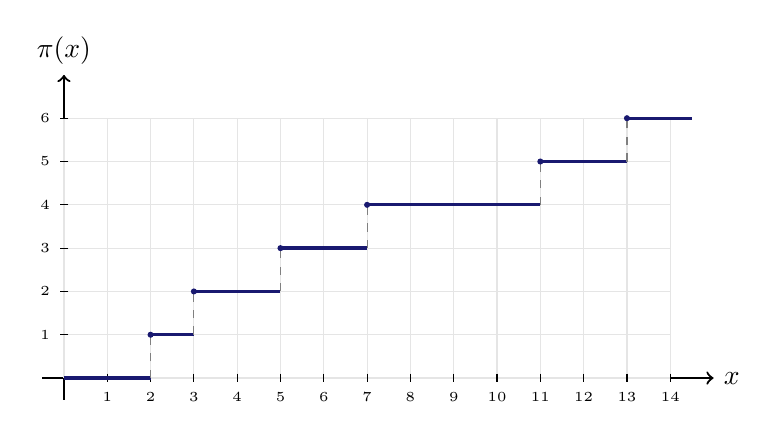
\begin{tikzpicture}[scale=0.55]
    \draw[->, thick] (-0.5,0) -- (15,0) node[right] {$x$};
    \draw[->, thick] (0,-0.5) -- (0,7) node[above] {$\pi(x)$};
    
    % Grid lines
    \draw[gray!20, thin] (0,0) grid (14,6);
    
    % Ticks
    \foreach \x in {1,2,...,14}
        \draw (\x, 0.1) -- (\x, -0.1) node[below] {\tiny $\x$};
    \foreach \y in {1,2,...,6}
        \draw (0.1, \y) -- (-0.1, \y) node[left] {\tiny \y};
        
    % Step function plot
    \draw[very thick, MidnightBlue] (0,0) -- (2,0);
    \draw[very thick, MidnightBlue] (2,1) -- (3,1);
    \draw[very thick, MidnightBlue] (3,2) -- (5,2);
    \draw[very thick, MidnightBlue] (5,3) -- (7,3);
    \draw[very thick, MidnightBlue] (7,4) -- (11,4);
    \draw[very thick, MidnightBlue] (11,5) -- (13,5);
    \draw[very thick, MidnightBlue] (13,6) -- (14.5,6);
    
    % Jumps (dashed)
    \draw[dashed, gray] (2,0) -- (2,1);
    \draw[dashed, gray] (3,1) -- (3,2);
    \draw[dashed, gray] (5,2) -- (5,3);
    \draw[dashed, gray] (7,3) -- (7,4);
    \draw[dashed, gray] (11,4) -- (11,5);
    \draw[dashed, gray] (13,5) -- (13,6);
    
    % Dots
    \fill[MidnightBlue] (2,1) circle (2pt);
    \fill[MidnightBlue] (3,2) circle (2pt);
    \fill[MidnightBlue] (5,3) circle (2pt);
    \fill[MidnightBlue] (7,4) circle (2pt);
    \fill[MidnightBlue] (11,5) circle (2pt);
    \fill[MidnightBlue] (13,6) circle (2pt);
\end{tikzpicture}
\end{center}
\end{math-stroke}

\begin{spoken-clean}[01:10:33 - 01:13:42]
Der Primzahlsatz, den wir hier aber nicht beweisen --- das ist viel zu schwierig ---, besagt, dass diese Funktion asymptotisch wie $x$ geteilt durch den natürlichen Logarithmus von $x$ wächst. Kennen Sie den Begriff \qt{asymptotisch}? Sagt Ihnen das was? Haben Sie verschiedene Wachstumsarten kennengelernt? Das heißt einfach: Wenn wir den Limes für $x$ gegen unendlich von $\pi(x)$ geteilt durch diese Funktion, also $x / \ln(x)$, nehmen, dann ist dieser Grenzwert $1$. Im Limes verhalten sich die beiden Funktionen also gleich. Die Anzahl der Primzahlen wächst im Wesentlichen wie $x / \ln(x)$, was intuitiv auch Sinn ergibt. Im Großen und Ganzen hat man das also verstanden.

Wenn Sie sich mit analytischer Zahlentheorie beschäftigen, begegnen Ihnen genau diese Fragen. Das Schöne ist, dass man diese Probleme mit Methoden der komplexen Analysis zusammenbringt. Meistens sind das Paper, in denen man auf $20$ Seiten komplizierte Integralabschätzungen durchführt, um am Schluss eine Fehlerschranke noch ein kleines bisschen zu verbessern --- sodass dort beispielsweise anstelle von plus $1/1000$ nun plus $1/2000$ steht. Aber genau darum geht es: diese Abschätzungen zu verfeinern. Wie Sie vielleicht wissen, gibt es noch bessere Näherungsfunktionen als $x / \ln(x)$, mit denen man das noch präziser beschreiben kann. Der genaue Fehlerterm, also wie weit die tatsächliche Anzahl von der Näherung abweicht, ließe sich mit der Riemannschen Vermutung sehr präzise bestimmen; bisher hat man da nur relativ grobe Abschätzungen. Gut, das machen wir hier aber nicht.
\end{spoken-clean}

\begin{math-stroke}[Der Primzahlsatz]
\begin{theorem}[Primzahlsatz]\label[theorem]{thm:primzahlsatz}
Die Primzahlzählfunktion $\pi(x)$ verhält sich asymptotisch wie $\frac{x}{\ln(x)}$:
\[ \pi(x) \sim \frac{x}{\ln(x)} \quad (x \to \infty) \]
Das bedeutet für den Grenzwert:
\[ \lim_{x \to \infty} \frac{\pi(x)}{\frac{x}{\ln(x)}} = 1 \]
\end{theorem}
\end{math-stroke}

\begin{didactic-insight}[Die Riemannsche Vermutung und der Fehlerterm]
Der Primzahlsatz beschreibt das globale, makroskopische Verhalten der Primzahlverteilung. Die mikroskopischen Abweichungen (der Fehlerterm $|\pi(x) - \operatorname{Li}(x)|$, wobei $\operatorname{Li}(x) = \int_2^x \frac{1}{\ln(t)} \, dt$ die noch präzisere logarithmische Integralfunktion ist) sind eng mit den Nullstellen der Riemannschen Zeta-Funktion $\zeta(s)$ verknüpft. Die berühmte Riemannsche Vermutung besagt, dass alle nicht-trivialen Nullstellen von $\zeta(s)$ den Realteil $\frac{1}{2}$ besitzen, was die bestmögliche Fehlerschranke für die Primzahlverteilung garantieren würde.
\end{didactic-insight}

\subsection{Die Eulersche \texorpdfstring{$\varphi$}{phi}-Funktion}

\begin{spoken-clean}[01:13:42 - 01:16:40]
Eine weitere Funktion, die ich definieren möchte --- und die wir uns nächste Woche noch etwas genauer anschauen werden ---, ist die berühmte eulersche $\varphi$-Funktion. Das ist eine Funktion, die von den positiven ganzen Zahlen in die positiven ganzen Zahlen geht (i.e., eigentlich von $\mathbb{N}_{>0}$ nach $\mathbb{N}_{>0}$), und sie ist wie folgt definiert: $\varphi(n)$ ist die Anzahl der natürlichen Zahlen $a$ zwischen $1$ und $n$, für die der größte gemeinsame Teiler von $a$ und $n$ gleich $1$ ist. Das ist eine sehr spannende Funktion.

Beispiel: $\varphi(1)$ ist einfach $1$, da gibt es nur die $1$. Und was ist $\varphi(2)$? Auch $1$, genau. Und $\varphi(3)$? Ja, $2$, genau. Sie dürfen übrigens einfach reinrufen, wenn Sie wollen. $\varphi(4)$? $2$, genau. Und $\varphi(6)$ ist ebenfalls $2$. Und allgemein für eine Primzahl $p$: Was ist $\varphi(p)$? Ja, genau $p - 1$. Für zusammengesetzte Zahlen wird es dann etwas komplizierter, das können wir uns später noch genauer anschauen.
\end{spoken-clean}

\begin{math-stroke}[Die Eulersche \texorpdfstring{$\varphi$}{phi}-Funktion]
\begin{definition}[Eulersche $\varphi$-Funktion]\label[definition]{def:euler-phi}
Die \newterm{Eulersche $\varphi$-Funktion} (auch Eulersche Indikatorfunktion) $\varphi \colon \mathbb{N}_{>0} \to \mathbb{N}_{>0}$ ordnet jeder Zahl $n \in \mathbb{N}_{>0}$ die Anzahl der zu $n$ teilerfremden natürlichen Zahlen $a$ mit $1 \le a \le n$ zu:
\[ \varphi(n) = \bigl| \{ a \in \mathbb{N} \mid 1 \le a \le n \land \operatorname{ggT}(a, n) = 1 \} \bigr| \]
\end{definition}

\begin{examples}[Berechnung von $\varphi(n)$]\label[examples]{ex:euler-phi-werte}
Wir berechnen einige Funktionswerte:
\begin{itemize}
    \item \textbf{$\varphi(1) = |\{1\}| = 1$} (da $\operatorname{ggT}(1,1) = 1$)
    \item \textbf{$\varphi(2) = |\{1\}| = 1$} (da $\operatorname{ggT}(1,2) = 1$, aber $\operatorname{ggT}(2,2) = 2$)
    \item \textbf{$\varphi(3) = |\{1, 2\}| = 2$} (da $3$ prim ist)
    \item \textbf{$\varphi(4) = |\{1, 3\}| = 2$} (da $\operatorname{ggT}(2,4) = 2$ und $\operatorname{ggT}(4,4) = 4$)
    \item \textbf{$\varphi(6) = |\{1, 5\}| = 2$} (da $2, 3, 4$ nicht teilerfremd zu $6$ sind)
\end{itemize}
Allgemein gilt für jede Primzahl $p \in \mathbb{N}$:
\[ \varphi(p) = p - 1 \]
\end{examples}
\end{math-stroke}

\section{Modularrechnen}
\subsection{Definition der Kongruenz}

\begin{spoken-clean}[01:16:40 - 01:18:25]
Okay, dann kommen wir zum nächsten Kapitel, das immer noch zur Zahlentheorie gehört. Das ist im Skript das Kapitel 11: Modularrechnen. Ich vermute mal, das haben Sie in der Linearen Algebra und der Analysis schon ein bisschen gemacht, aber vielleicht noch nicht so ausführlich. Das schauen wir uns jetzt auf jeden Fall gründlich an, weil es in der Mathematik extrem wichtig ist und immer wieder gebraucht wird.

Wir sagen, dass zwei ganze Zahlen $a$ und $b$ kongruent modulo $n$ sind, falls $n$ ein Teiler der Differenz $a - b$ ist. Weil man das so oft verwendet, haben wir dafür eine eigene Notation: Wir schreiben $a \equiv b \pmod n$ (gesprochen: $a$ ist kongruent zu $b$ modulo $n$).

Okay, und da gibt es verschiedene Möglichkeiten, das zu interpretieren. Als Bemerkung: Wir sehen, dass $a \equiv b \pmod n$ genau dann gilt, wenn sich $a$ und $b$ nur um ein ganzzahliges Vielfaches von $n$ unterscheiden. Das heißt, wir können schreiben: $a = b + k \cdot n$ für ein $k \in \mathbb{Z}$. Die Differenz ist also ein Vielfaches von $n$. Und das wiederum ist äquivalent zu der Aussage, dass $a$ und $b$ bei Division durch $n$ denselben Rest ergeben. Wir betrachten die Zahlen hier also im Wesentlichen nur bis auf Vielfache von $n$.
\end{spoken-clean}

\begin{math-stroke}[Definition der Kongruenz]
\begin{definition}[Kongruenz modulo $n$]\label[definition]{def:kongruenz}
Sei $n \in \mathbb{Z}$ \inlinemetanote{[Anmerkung: Meistens schließt man $n=0$ aus (wie in der folgenden Proposition), obwohl die Teilbarkeitsbedingung formal auch für $n=0$ als $a=b$ auswertbar wäre]} und seien $a, b \in \mathbb{Z}$. Wir sagen, $a$ und $b$ sind \newterm{kongruent modulo $n$}, falls $n$ die Differenz $a - b$ teilt:
\[ n \mid (a - b) \]
Notation: $a \equiv b \pmod n$.
\end{definition}

\begin{proposition}[Charakterisierung der Kongruenz]\label[proposition]{prop:kongruenz-charakterisierung}
Für $a, b, n \in \mathbb{Z}$ mit $n \neq 0$ sind folgende Aussagen äquivalent:
\begin{enumerate}[label=\textbf{(\roman*)}]
    \item $a \equiv b \pmod n$.
    \item Es existiert ein $k \in \mathbb{Z}$, sodass $a = b + k \cdot n$.
    \item Bei Division von $a$ und $b$ durch $n$ mit Rest ergibt sich derselbe Rest.
\end{enumerate}
\end{proposition}
\end{math-stroke}

\subsection{Kongruenz als Äquivalenzrelation}

\begin{math-stroke}[Kongruenz als Äquivalenzrelation]
\begin{proposition}[Äquivalenzrelation]\label[proposition]{prop:kongruenz-aequivalenzrelation}
Die Relation der Kongruenz modulo $n$ ist eine Äquivalenzrelation auf $\mathbb{Z}$.
\end{proposition}
\end{math-stroke}

\begin{proof}[Beweis von \cref{prop:kongruenz-aequivalenzrelation}]
\begin{spoken-clean}[01:18:25 - 01:20:46]
Die wichtige Bemerkung ist: Das definiert eine Äquivalenzrelation auf $\mathbb{Z}$. Okay, das können wir zeigen. Wir müssen zeigen, dass die Relation reflexiv, symmetrisch und transitiv ist. Zuerst die Reflexivität: Wir sehen, dass $a \equiv a \pmod n$ gilt. Ich meine, das ist klar, weil jede Zahl ein Teiler von $0$ ist.

Dann wissen wir, dass die Relation symmetrisch ist. Falls $a \equiv b \pmod n$ gilt, dann teilt $n$ die Differenz $a - b$. Aber dann teilt $n$ natürlich auch $b - a$. Und somit gilt auch $b \equiv a \pmod n$. Das ist sehr direkt.

Und das Dritte ist ebenfalls direkt: die Transitivität. Falls $a \equiv b \pmod n$ und $b \equiv c \pmod n$ gilt, dann folgt, dass $n \mid (a - b)$ und $n \mid (b - c)$ gilt. Daraus folgt aber, dass $n$ auch die Summe der beiden teilt (d.\,h. $(a - b) + (b - c) = a - c$). Das heißt, $n \mid (a - c)$, und somit gilt $a \equiv c \pmod n$.

Gut, okay. Da wir nun eine Äquivalenzrelation haben, bedeutet das, dass unser $\mathbb{Z}$ in Äquivalenzklassen zerfällt. Wir erhalten eine Partition von $\mathbb{Z}$ in Äquivalenzklassen. Für jedes $a \in \mathbb{Z}$ bezeichnen wir mit $\bar{a}$ die Äquivalenzklasse von $a$ modulo $n$. Das heißt, $\bar{a}$ ist die Menge aller ganzen Zahlen $x \in \mathbb{Z}$, die kongruent zu $a$ modulo $n$ sind --- also alle $x$, sodass $n$ ein Teiler von $x - a$ ist.
\end{spoken-clean}

\begin{math-stroke}[Beweis der Äquivalenzrelation]
Wir verifizieren die drei definierenden Axiome:
\begin{itemize}
    \item \textbf{Reflexivität:} Für alle $a \in \mathbb{Z}$ gilt $a - a = 0$. Da $n \mid 0$, folgt $a \equiv a \pmod n$.
    \item \textbf{Symmetrie:} Gilt $a \equiv b \pmod n$, so gilt $n \mid (a - b)$. Daraus folgt $n \mid -(a - b) = b - a$, also $b \equiv a \pmod n$.
    \item \textbf{Transitivität:} Gilt $a \equiv b \pmod n$ und $b \equiv c \pmod n$, so gilt $n \mid (a - b)$ und $n \mid (b - c)$. Dann teilt $n$ auch deren Summe:
    \[ n \mid \bigl( (a - b) + (b - c) \bigr) = a - c \implies a \equiv c \pmod n \]
\end{itemize}
\end{math-stroke}
\end{proof}

\begin{math-stroke}[Definition der Restklasse]
\begin{definition}[Restklasse]\label[definition]{def:restklasse}
Die Äquivalenzklassen bezüglich der Kongruenz modulo $n$ heißen \newterm{Restklassen} (oder \newterm{Kongruenzklassen}). Für $a \in \mathbb{Z}$ bezeichnen wir die Restklasse von $a$ mit:
\[ \bar{a} := \{ x \in \mathbb{Z} \mid x \equiv a \pmod n \} = \{ x \in \mathbb{Z} \mid n \mid (x - a) \} \]
Die Menge aller Restklassen modulo $n$ wird mit $\mathbb{Z}/n\mathbb{Z}$ bezeichnet.
\end{definition}
\end{math-stroke}

\subsection{Verträglichkeit mit den Ringoperationen}

\begin{math-stroke}[Verträglichkeit der Kongruenz mit Addition und Multiplikation]
\begin{lemma}[Verträglichkeit]\label[lemma]{lem:vertraglichkeit}
Seien $a, b, a', b' \in \mathbb{Z}$ mit $a \equiv a' \pmod n$ und $b \equiv b' \pmod n$. Dann gilt:
\begin{align}
    a + b &\equiv a' + b' \pmod n \label{eq:vertraglichkeit-add} \\
    a \cdot b &\equiv a' \cdot b' \pmod n \label{eq:vertraglichkeit-mul}
\end{align}
\end{lemma}
\end{math-stroke}

\begin{proof}[Beweis von \cref{lem:vertraglichkeit}]
\begin{spoken-clean}[01:20:46 - 01:21:27]
Okay. Und das Schöne ist jetzt --- auch wenn es vielleicht ein bisschen Rechnerei ist ---: Diese Relation ist verträglich mit der Addition und der Multiplikation. Das ist das folgende Lemma.

Der Beweis ist eine direkte Rechnung. Falls $n \mid (a - a')$ und $n \mid (b - b')$ gilt, dann folgt daraus, dass $n$ auch die Summe dieser Differenzen teilt, also $(a - a') + (b - b')$. Das kann man einfach umschreiben als $(a + b) - (a' + b')$. Das bedeutet genau, dass $a + b \equiv a' + b' \pmod n$ gilt.

Und ganz ähnlich machen wir es für die Multiplikation. Wenn $n \mid (a - a')$ und $n \mid (b - b')$ gilt, dann folgt, dass $n$ auch den folgenden Term teilt --- lassen Sie mich hier kurz den richtigen Term wählen ---: $(a - a') \cdot b + a' \cdot (b - b')$. Wenn $n$ die einzelnen Faktoren teilt, dann teilt es auch deren Vielfache, und folglich teilt es auch die Summe dieser beiden Summanden. Wenn man diesen Ausdruck nun ausrechnet, ergibt das einfach $a \cdot b - a' \cdot b'$. Und somit haben wir gezeigt, dass $a \cdot b \equiv a' \cdot b' \pmod n$ gilt. Okay, und das beendet den Beweis.

In anderen Worten: Sie können Repräsentanten der Äquivalenzklassen miteinander addieren oder multiplizieren, und es spielt keine Rolle, welche Repräsentanten Sie wählen --- es kommt am Ende immer dieselbe Äquivalenzklasse heraus. Das werden wir uns nächste Woche noch genauer anschauen. Okay, gibt es dazu noch Fragen? Gut, dann höre ich für heute hier auf. Machen Sie auf jeden Fall das Aufgabenblatt für diese Woche; es sind wieder sehr nette Aufgaben, diesmal zum Schubfachprinzip, dabei. Das ist eine hervorragende Übung, und das Schubfachprinzip sollten Sie auf jeden Fall beherrschen. Vielen Dank fürs Kommen und bis nächste Woche!
\end{spoken-clean}

\begin{math-stroke}[Beweis der Verträglichkeit]
Nach Voraussetzung gilt $n \mid (a - a')$ und $n \mid (b - b')$.
\begin{itemize}
    \item \textbf{Beweis für die Addition:}
    Da $n$ beide Differenzen teilt, teilt $n$ auch deren Summe:
    \[ n \mid \bigl( (a - a') + (b - b') \bigr) \implies n \mid \bigl( (a + b) - (a' + b') \bigr) \]
    Dies zeigt unmittelbar die Behauptung \eqref{eq:vertraglichkeit-add}.
    
    \item \textbf{Beweis für die Multiplikation:}
    Wir betrachten die algebraische Identität:
    \[ a \cdot b - a' \cdot b' = (a - a') \cdot b + a' \cdot (b - b') \]
    Da $n \mid (a - a')$, teilt $n$ auch den ersten Summanden $(a - a') \cdot b$.
    Da $n \mid (b - b')$, teilt $n$ auch den zweiten Summanden $a' \cdot (b - b')$.
    Folglich teilt $n$ die gesamte Summe, was $n \mid (a \cdot b - a' \cdot b')$ und somit \eqref{eq:vertraglichkeit-mul} beweist.
\end{itemize}
\end{math-stroke}
\end{proof}

\begin{nice-box}[Zusammenfassung der Schlüsselkonzepte]
In dieser Vorlesung haben wir die Grundlagen der elementaren Zahlentheorie erarbeitet:
\begin{itemize}
    \item \textbf{Teilbarkeit \& Division mit Rest:} Für alle $a \in \mathbb{N}_{>0}, b \in \mathbb{Z}$ existieren eindeutige $q, r \in \mathbb{Z}$ mit $b = a \cdot q + r$ und $0 \le r < a$.
    \item \textbf{Größter gemeinsamer Teiler ($\operatorname{ggT}$):} Der $\operatorname{ggT}(a, b)$ ist der eindeutige gemeinsame Teiler, der von jedem anderen gemeinsamen Teiler geteilt wird. Er lässt sich als Linearkombination $d = a \cdot x + b \cdot y$ darstellen (Lemma von Bézout).
    \item \textbf{Euklidischer Algorithmus:} Ein sukzessives Divisionsverfahren zur effizienten Berechnung des $\operatorname{ggT}(a, b)$ als letzter von Null verschiedener Rest $r_n$.
    \item \textbf{Hauptsatz der Arithmetik:} Jede ganze Zahl $a \neq 0$ besitzt eine bis auf die Reihenfolge eindeutige Primfaktorzerlegung $a = c \cdot p_1 \cdots p_k$ mit $c \in \{1, -1\}$.
    \item \textbf{Satz von Euklid:} Es existieren unendlich viele Primzahlen.
    \item \textbf{Eulersche $\varphi$-Funktion:} Bestimmt die Anzahl der zu $n$ teilerfremden Zahlen $a$ mit $1 \le a \le n$. Für Primzahlen gilt $\varphi(p) = p - 1$.
    \item \textbf{Modularrechnen:} Die Kongruenz $a \equiv b \pmod n$ definiert eine Äquivalenzrelation auf $\mathbb{Z}$, deren Klassen (Restklassen) wohldefinierte Additionen und Multiplikationen erlauben.
\end{itemize}
\end{nice-box}

% [SYSTEM] Video complete.